\chapter{Introduction and background}
\label{chap:intro}

In this chapter, we will discuss the basics of protein and ligand-binding sites problematic, later in this chapter will we cover the current PrankWeb architecture and the P2Rank tool itself. The reader will also be briefly introduced to similar web-tools.

\section{Introduction to molecular biology}
\label{sec:mol_bio}

\xxx{TODO}
\xxx{mention keywords: protein, ligand, binding site, pocket, docking, conservation, prediction, structure, residues, sequence, amino acids}

\section{P2Rank tool}
\label{sec:p2rank}

P2Rank allows its users to predict the ligand-binding sites for a given protein. In contrast to other projects, P2Rank was one of the first tools to employ machine learning for predicting the pockets. P2Rank outperforms most of the existing binding sites prediction tools \cite{krivak2018p2rank}. Most of the other tools include geometry-based, energetic-based, or template-based methods that are not as efficient and rather outdated. Moreover, P2Rank works as a standalone application and is fully automated, which makes the tool very intuitive and easy to use.

P2Rank works with specific file formats such as PDB and PDBx/mmCIF. \xxx{maybe insert some detailed explanation of the formats including JSON, or add a footnote?} After running the tool on a specific protein structure file, the tool will provide a CSV output file with the prediction and residue-level scores. The output file includes predicted pockets, their ranks, center coordinates, adjacent residues, related surface atoms and a probability score.

The following command would run P2Rank on the protein structure file \texttt{1fbl.pdb}:

\begin{Verbatim}
    prank predict -f test_data/1fbl.pdb 
\end{Verbatim}

The tool was written in Java and requires only the JRE\footnote{Java Runtime Environment.} to run. Additionally, the source codes are publicly available at GitHub\footnote{Source codes for P2Rank are available at \url{https://github.com/rdk/p2rank}.}. This allows the users to potentially modify the tool to their respective needs. 

\section{PrankWeb architecture}
\label{sec:prankweb_arch}

PrankWeb consists of several components that cooperate together. Currently, the application is deployed via Docker\footnote{Docker is a virtualization tool providing a stable interface for isolating and running applications. More information available at \url{https://www.docker.com/}.} containers that are described in the \texttt{docker-compose.yml} file. The application consists of the following components:

\begin{itemize}
    \item \textbf{gateway} - a reverse proxy that is responsible for routing the requests to the respective backend services
    \item \textbf{rabbitmq} - a broker that is used for communication between the gateway and the backend services
    \item \textbf{flower} - a tool for monitoring the RabbitMQ broker and Celery workers
    \item \textbf{web-server} - a WSGI server that is responsible for serving the web application
    \item \textbf{executor-p2rank} - a backend service that is responsible for running the P2Rank tool, employs Celery workers
    \item \textbf{executor-docking} - a backend service that is responsible for running the docking tool, employs Celery workers \xxx{docking not done yet though}
    \item \textbf{prometheus} - a tool for monitoring the Docker containers 
\end{itemize}

\xxx{TODO: add a diagram of the architecture}

Some of the containers include environment variables that are required for the proper functionality. The environment variables are specified in the \texttt{docker-compose.yml} file. The user may modify these also by creating a \texttt{.env} file in the root directory of the project.

The \texttt{docker-compose.yml} file thus contains the entire PrankWeb logic. When employing a new plug-in or a new feature, a container may be introduced to this file to get easily integrated into the application.

Each of the containers is defined by a respective \texttt{Dockerfile}. Some containers are dependent on the order of deployment, some containers include a Docker volume definition that ensures the persistence of the data.

Now we will present the current Docker containers in more detail to get a broader knowledge of the architecture.

\subsection{Gateway}
\label{subsec:gateway}

The gateway container is a reverse proxy that is responsible for routing the requests to the backend. In PrankWeb, we utilize the Nginx web server as a reverse proxy. The Nginx configuration file is located in the \texttt{gateway/nginx.conf} file. The server configuration includes not only the reverse proxy routes, but a mapping to the Flower and Prometheus services as well.

Moreover, \texttt{gateway/Dockerfile} is responsible for the installation of the frontend. The frontend is a React application built via webpack. PrankWeb utilizes two main external libraries for the bioinformatic part of the application, MolStar and RCSB Saguaro Feature 1D Viewer. We will discuss these libraries in more detail in the next chapter.

The entire frontend is written in TypeScript, JavaScript, CSS, SCSS, and HTML.

\subsection{RabbitMQ}
\label{subsec:rabbitmq}

RabbitMQ is a message broker that is used to provide communication between the web server and the backend workers, in our case Celery. RabbitMQ is configured via the \texttt{rabbitmq/rabbitmq/rabbitmq.conf} file. PrankWeb does not require a complex configuration of this service, although the service is still necessary for the communication.

\subsection{Flower}
\label{subsec:flower}

Flower is a tool for monitoring the broker and Celery workers functionality. Flower container does not need any specific configuration, it is only necessary to correctly run it alongside the RabbitMQ container.

\subsection{Web-server}
\label{subsec:web-server}

The web-server container is a WSGI server that is responsible for serving the web application. Currently, we employ the Gunicorn server. The second main part of this continer is Flask framework. The Flask application defines all of the REST API endpoints for interaction between the frontend and the backend. This application also defines a Celery client that is responsible for sending the tasks to the backend Celery workers based on the API calls.

\subsection{Executor-P2Rank}
\label{subsec:executor-p2rank}

This container is responsible for creating the prediction via the P2Rank tool. P2Rank executor is written in Python and utilizes the Celery framework for the task management. Celery enables the server to use multiple threads and process the requests in parallel. The executor's Celery listener firstly receives a request for the prediction given a directory with a name of the structure. Subsequently, the executor prepares the necessary information for the P2Rank tool.

The tool is then run and the results are saved in the

\texttt{predictions/<db-name>\footnote{Represents the current version of database such as v2, v3,  v3-alphafold, v3-conservation-hmm etc.}/<structure-short>\footnote{The shortcut consists of second two letters of the structure identifier, i.e \texttt{SR} for \texttt{2SRC} or \texttt{5V} for \texttt{Q5VSL9}.}/<structure-name>} 

directory. The current hierarchy contains the following:
\begin{itemize}
    \item \texttt{input/configuration.json} - a JSON file required for a configuration of the P2Rank tool, containing the structure code, name of the structure file, conservation and others
    \item \texttt{public/structure.cif.gz} - a gzipped\footnote{Gzip is an Unix-based tool for file compression.} mmCIF/PDB file of the structure
    \item \texttt{public/prediction.json} - a JSON file containing the prediction results derived from the P2Rank tool specifically for easier parsing in the frontend
    \item \texttt{public/prankweb.zip} - a zip file containing unmodified, verbose output files directly from the P2Rank tool
    \item \texttt{info.json} - a JSON file containing current prediction status
    \item \texttt{log} - a log file containing the output of the P2Rank tool
\end{itemize}

All of the listed files are exposed via the REST API to the frontend. After posting a prediction request, the frontend periodically polls the \texttt{info.json} file to get the current status of the prediction. Meanwhile, the \texttt{log} file is continuously updated with the output of the P2Rank tool. The logfile is also shown in the frontend to provide the user with the current status of the prediction.

\subsection{Executor-Docking}
\label{subsec:executor-docking}

\xxx{TODO - not implemented yet, but the idea is pretty much the same as for the P2Rank executor}

\subsection{Prometheus}
\label{subsec:prometheus}

Prometheus is a tool for monitoring the Docker containers. It is not necessary for the proper application functionality, but is useful for debugging purposes. The Prometheus container is configured via the \texttt{prometheus/prometheus.yml} file. The interface is exposed at the \texttt{9090} port.

\section{Similar web-tools}
\label{sec:similar_web_tools}

The main motivation for the creation of PrankWeb was to provide a web-based ligand binding site prediction tool that does employ the newest technologies not only for the prediction itself, but also for the web application. One of the goals of this thesis is to replace the outdated plugins for the structure, pockets and binding sites visualization to keep the application relevant and up-to-date.

There are a few working web-tools that are able to predict binding sites for the structure as well. The main issue with these tools is that most of them are utilizing outdated technologies and do not appear to be as intuitive as PrankWeb\cite{jendele2019prankweb}. Moreover, PrankWeb focuses on the visual side of the prediction and provides a more detailed view of the results, while the other tools are relying on the user to interpret the downloadable results in other tools such as PyMOL.

We will cover a few of the existing web-tools to provide a better understanding of the current state of the art.

\subsection{IntFOLD}
\label{subsec:intfold}

IntFOLD\footnote{Available at \url{https://www.reading.ac.uk/bioinf/IntFOLD/}.} is a tool that may be used for predicting protein tertiary structures alongside disordered protein regions and ligand binding sites. This tool utilizes the FunFOLD algorithm to create the predictions effectively \cite{10.1093/nar/gkz322}. IntFOLD appears to be still actively developed and is easily accessible to any potential user. The user interface is easy to use and requires only the protein sequence (FASTA) to be entered. On the other side, IntFOLD uses the JSMol library for visualising the protein binding sites. JSMol is more of a simple viewer with less options than the MolStar library used in PrankWeb. Both the visuals and the user interaction are limited. The user may modify the representation with a right mouse button click, but the interface is pretty complicated and non-intuitive. An example prediction is shown in Figure \ref{fig:intfold_prediction}. Like PrankWeb, IntFOLD also provides a download option for the prediction results for PyMOL. The prediction takes a long time to be computed, typically around 24 hours.

\begin{figure}
    \centering
    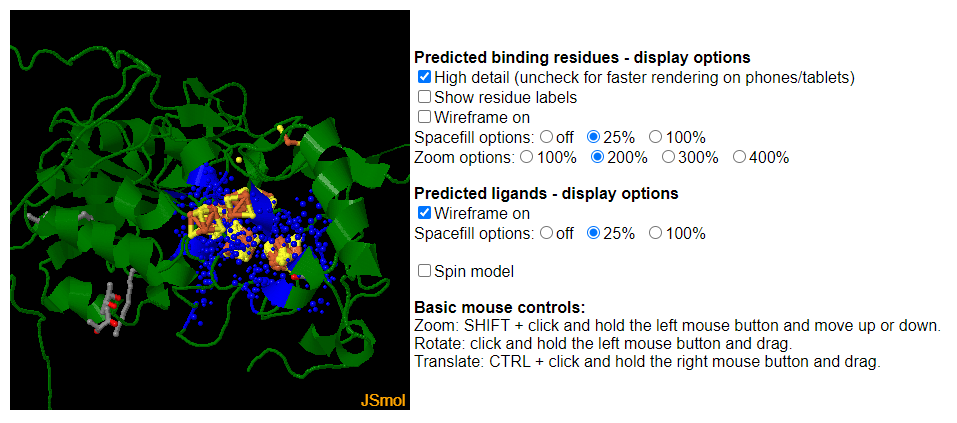
\includegraphics[width=\linewidth]{img/intfold_prediction.png}
    \caption{JSmol view of ligand binding residues prediction for T1114s2.
    Available at \url{https://www.reading.ac.uk/bioinf/servlets/nFOLD/IntFOLD7results.jsp?time=17_8_50_25_11-5-2022_CASP_ALL_mesu41b7re376c8l&md5=mesu41b7re376c8l&targetname=T1114s2}. The structure is shown in dark green, the binding sites prediction is shown in blue. Predicted ligands are shown yellow-orange. Available as a sample prediction from IntFOLD.}
    \label{fig:intfold_prediction}
\end{figure}

\subsection{COACH}
\label{subsec:coach}

COACH\footnote{Available at \url{https://seq2fun.dcmb.med.umich.edu/COACH/}} is a web-based tool designed specifically for binding sites prediction, like PrankWeb. COACH uses a combination of substructure-comparison (TM-Site) and sequence-alignment (S-Site) methods for the computations \cite{yang2013protein}. These methods are generally slower than the P2Rank tool, so the prediction once again is available to the user after a longer time, typically around 24 hours. This tool allows the user not only to enter a FASTA sequence, but also to upload or paste a PDB file. COACH allows the user to download the prediction results as well and does not focus on the web visualization that is very limited. An example prediction is shown in Figure \ref{fig:coach_prediction}.

\begin{figure}
    \centering
    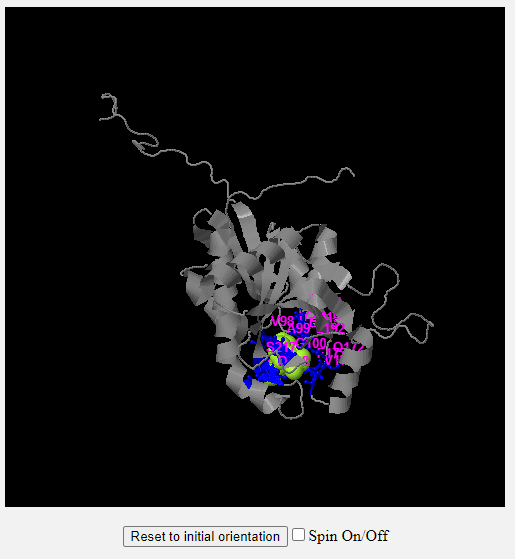
\includegraphics[width=.75\linewidth]{img/coach_prediction.png}
    \caption{JSmol view of a COACH prediction result for a sample protein available at \url{https://seq2fun.dcmb.med.umich.edu/COACH/CH000001/}. Compared to IntFOLD, the structure has implicitly less details and the user may change the representation only with a right mouse button click via JSMol settings.}
    \label{fig:coach_prediction}
\end{figure}

\subsection{DeepSite}
\label{subsec:deepsite}

DeepSite\footnote{Available at \url{https://www.playmolecule.com/deepsite/}} is one of the newest tools for binding sites prediction. DeepSite is a part of PlayMolecule framework that aims at the visual representation of the protein structures and their interactions. DeepSite uses machine-learning based methods to precisely predict the binding sites, which makes the tool very fast \cite{10.1093/bioinformatics/btx350}. The waiting times are significantly slower and the prediction is available to the user after a few minutes. The user may enter the PDB structure ID, which is a lot more convenient way to describe the structure than by entering the entire PDB file. DeepSite utilizes the MolStar library for the results and is similar to PrankWeb in terms of the visual representation. On the other side, DeepSite provides the user only with a visualisation of the center of the binding site and does not provide any information about the residues that are involved in the binding directly in the web viewer. The structure is shown in a surface representation. An example prediction is shown in Figure \ref{fig:deepsite_prediction}. The pros of this tool are definitely the speed of the prediction and a above-average visual representation. On the other side, the user is provided with little information about the binding site and may be used for a rather quick overview of the potential binding sites.

\begin{figure}
    \centering
    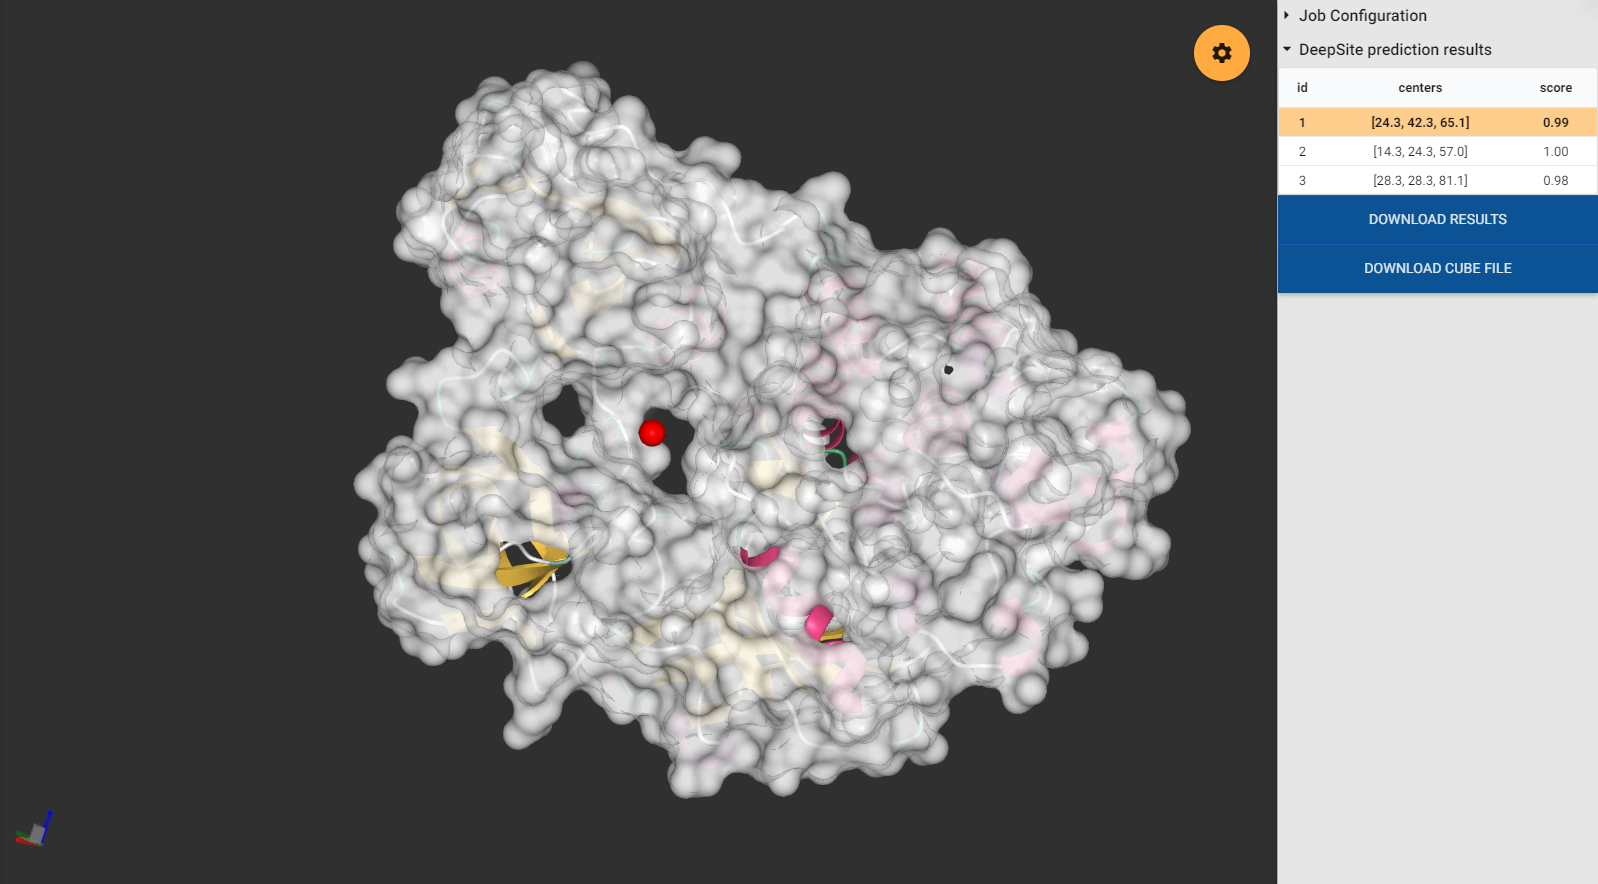
\includegraphics[width=\linewidth]{img/deepsite_prediction.png}
    \caption{A DeepSite prediction for the \texttt{2SRC} structure available at \url{https://www.playmolecule.com/deepsite/job/BD2ED307}. The surface representation is shown in white, underlying cartoon representation is colorful. The binding site prediction is shown by a red sphere.}
    \label{fig:deepsite_prediction}
\end{figure}